\section{Segmentation}
\label{sec:warmup5}

    We were given chest X-ray images of patients, and the segment masks of lungs. We need to employ a deep learning model that can generate segment masks of lungs

\subsection{Dataset}

    \begin{figure}
        \centering
        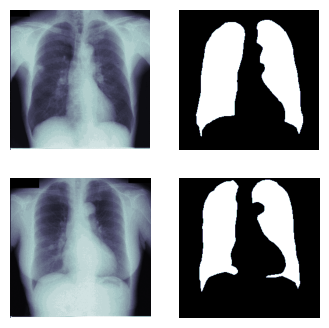
\includegraphics[width=\linewidth]{images/sample-segmentations.png}
        \caption{Chest XRays with lung segmentation masks}
        \label{fig:sample-segmentations}
    \end{figure}

    The provided dataset have $50$ training x-ray images and $10$ testing images, with their corresponding masks as shown in \cref{fig:sample-segmentations}, thus the provided dataset is very small. As there was no validtion set, I have randomly splited the training dataset into validation and training set in ration 1:9 respictively. The images in this dataset were color image with shape $256$x$256$, which is resized to image of size $64$x$64$.

\subsection{Training}

    This being a segmentation problem, an encoder-decoder type of model needs to be employed. I have created a UNet as shown in \cref{fig:unet_lung}. The model have a encoder block and a decoder block. There's also a skip connection which will allow the model to skip the decoder block. The model is trained using mean square error function with Adam optimizer having a learning rate of $0.003$. \Cref{fig:unet-learning-curve} illustrates the learning curve of the training and validation sets.

    \begin{figure}[htbp]
        \centering
        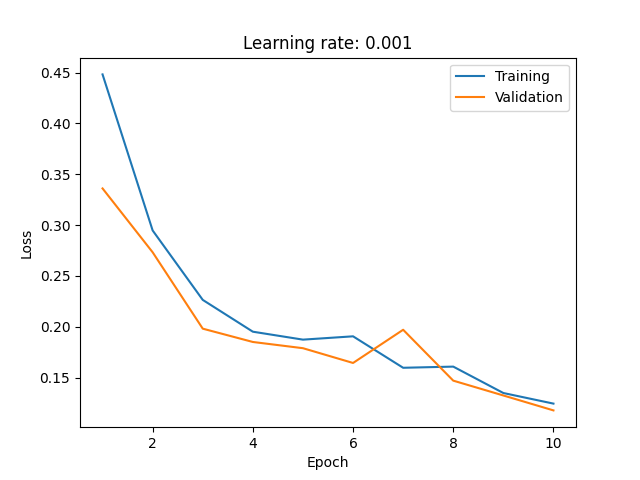
\includegraphics[width=\linewidth]{../outputs/segmentation/Segmentation01A/loss-curve.png}
        \caption{UNet model learning curve on training and validation sets}
        \label{fig:unet-learning-curve}
    \end{figure}

\subsection{Results}

    The model seems to converge to minimum loss as seen in \cref{fig:unet-learning-curve}. The IoU and DICE score of the model doesn't reflect the model performance, thus I haven't shared the scores. 